% !TeX root = d2.tex

\documentclass{article}

\usepackage{xcolor}
\usepackage[margin=0.5in]{geometry} 
\usepackage{graphicx}
\title{MindMerge --- Deliverable e 2}
\author{Gabriele Benetti, Gioele Bernardini, Luca Fossa Crescini, Luca Sartore}

\begin{document}
\maketitle


\tableofcontents


\newpage
\section*{Abstract}   % titolo temporaneo da modificare
This is the Abstract of the deliverable 2

\section{Architecture description}


\begin{figure}[h]
  \centering
  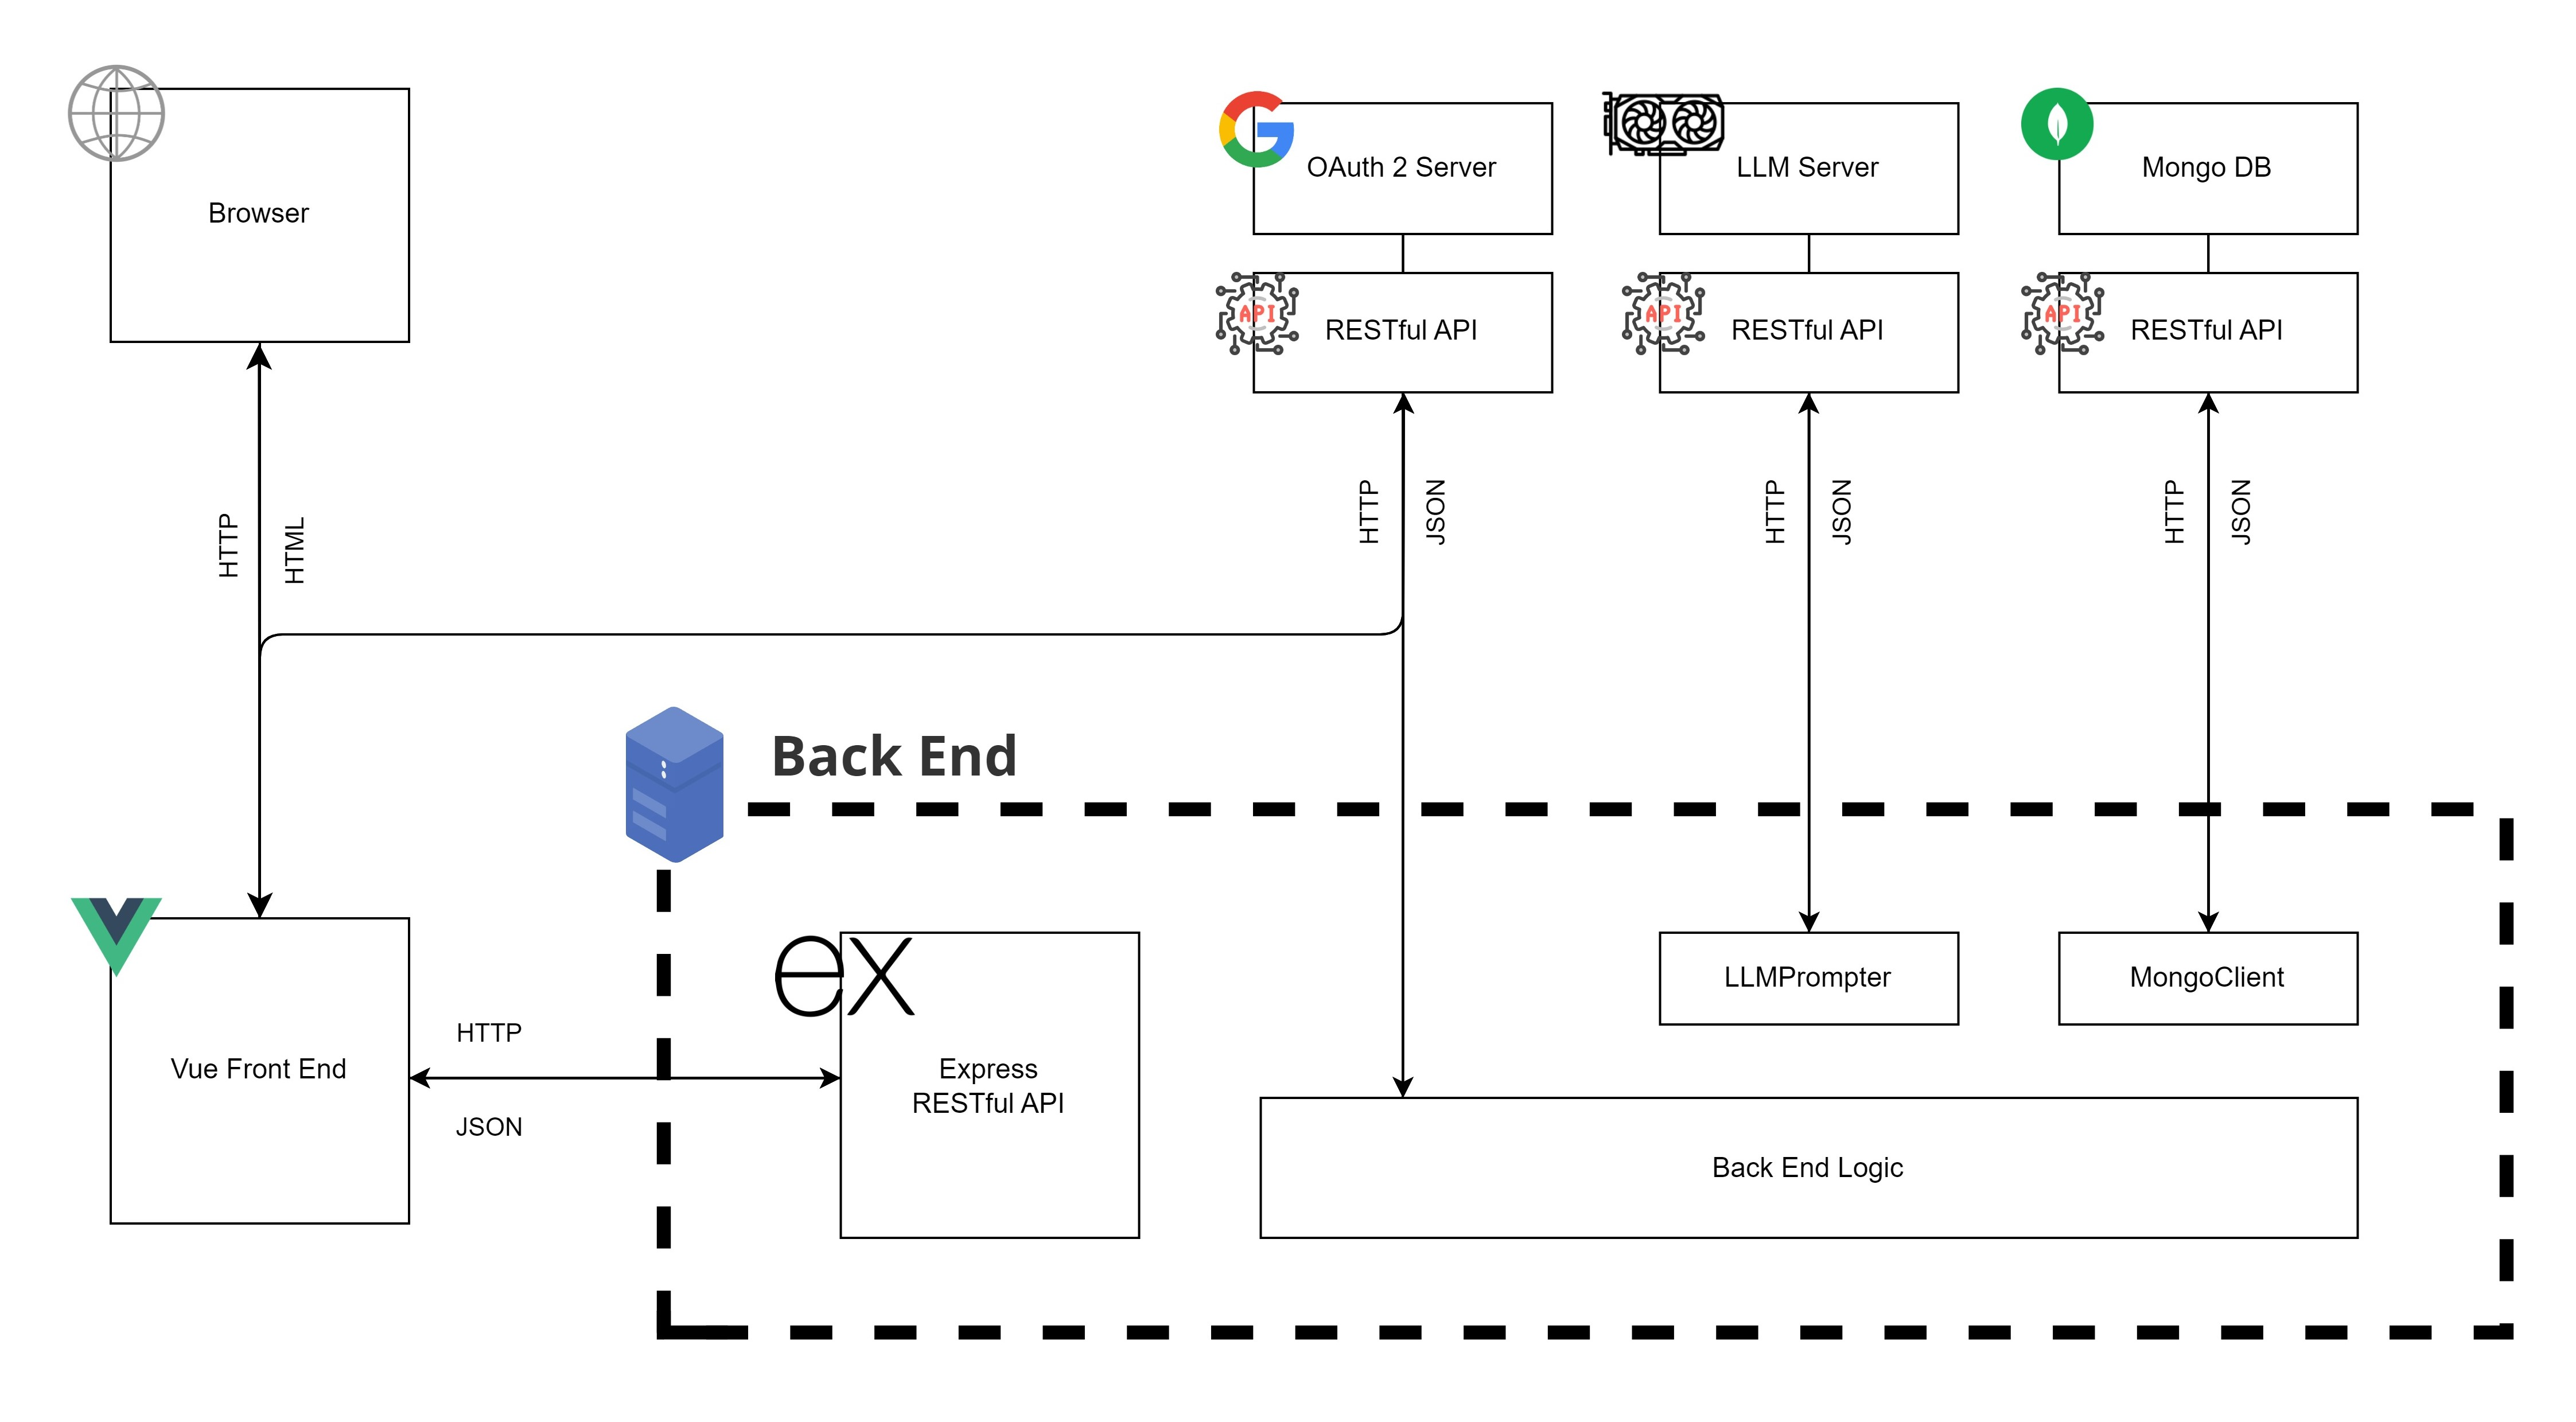
\includegraphics[width=0.95\textwidth]{images/architecture.jpg}
  \caption{\small The architecture diagram ot the MindMerge system}
\end{figure}
The architecture is relatively simple,
comprising two classical components: the front end and the back end, along with several smaller components (browser, OAuth server, LLM service, and MongoDB).
\newline \newline
The browser communicates with the front end using the HTTP protocol and HTML format.
\newline \newline
The front end, based on the Vue library, accesses resources provided by the back end using HTTP with JSON data format.
\newline \newline
Authentication is provided by a third-party OAuth server, that communicate with both the front end and back end via HTTP/JSON.
\newline \newline
The back end is the most complex component consists of several sub-components, including:
\begin{itemize}
    \item A part providing RESTful APIs based on Express.js
    \item A component dedicated to communicating with the database (MongoClient)
    \item A module for communicating with the LLM service (LLMPrompter)
    \item Logic containing all functions necessary for the application's operation.
\end{itemize}
All the communications that the backend has with the external world are made through HTTP with json format.
\end{document}

\end{document}